\documentclass[a4paper,11pt]{article}

\usepackage[utf8]{inputenc} % Unicode support (Umlauts etc.)
\usepackage[ngerman]{babel} % Change hyphenation rules
\usepackage{ziffer} % , können in Zahlen verwendet werden ohne Formatierung kaputt zu machen
\usepackage[top=30mm,right=20mm,bottom=15mm,left=25mm,includefoot,headheight=32pt]{geometry} % Seitenränder

\usepackage{lmodern,textcomp} % The package supports the Text Companion fonts, which provide many text symbols (benötigt für €)
\usepackage[fleqn]{amsmath} % Formatierte Gleichungen
\usepackage{graphicx} % Grafiken
\usepackage{xcolor} % Farbe in Text
\usepackage{fancyhdr} % Seitenstil mit Kopfzeile etc.

\usepackage{cases} % Fallunterscheidungen mathematisch uebereinander

\usepackage{floatflt}

\pagestyle{fancy}
\fancyhf{}
\lhead{
    Lösung \\
    Übungsblatt 6
}
\rhead{Gruppe 3 \\Nils \textbf{Hodys}, Sascha \textbf{Majewsky}}
\rfoot{Seite \thepage}

\setlength{\parindent}{0cm} % Keine Einrückung der 1. Zeile eines Absatzes

\begin{document}

\raggedright % Alles Linksbündig

\section*{Aufgabe 1}
\subsection*{1.}
\begin{align*}
& A \land \neg (\neg B \to C) & \\
\Leftrightarrow & A \land \neg (B \lor C) && \big| \text{Implikation auflösen} \\
\Leftrightarrow & A \land \neg B \land \neg C && \big| \text{De-Morgan} \\
\end{align*}

\subsection*{2.}
\begin{align*}
& A \to B \land \neg (C \lor D) & \\
\Leftrightarrow & \neg A \lor B \land \neg (C \lor D) && \big| \text{Implikation auflösen} \\
\Leftrightarrow & \neg A \lor (B \land \neg C \land \neg D) && \big| \text{De-Morgan \& Klammer f. Sichtbarkeit setzen} \\
\Leftrightarrow & (\neg A \lor B) \land (\neg A \lor \neg C) \land (\neg A \lor \neg D) && \big| \text{Distributivgesetz anwenden}
\end{align*}

\subsection*{3.}
\begin{align*}
& \neg(\neg A \land B) \lor (C \leftrightarrow D) & \\
\Leftrightarrow & \neg(\neg A \land B) \lor ((C \to D) \land (D \to C)) && \big| \text{Äquivalenz zu Implikationen} \\
\Leftrightarrow & \neg(\neg A \land B) \lor ((\neg C \lor D) \land (\neg D \lor C)) && \big| \text{Implikationen auflösen} \\
\Leftrightarrow & A \lor \neg B \lor ((\neg C \lor D) \land (\neg D \lor C)) && \big| \text{De-Morgan} \\
\Leftrightarrow & (A \lor \neg B \lor \neg C \lor D) \land (A \lor \neg B \lor \neg D \lor C) && \big| \text{Distributivgesetz anwenden}
\end{align*}


\section*{Aufgabe 2}
\begin{align*}
\textbf{1. } & P2 \to P3 \\
\Leftrightarrow & \neg P2 \lor P3 \\
\Rightarrow  & (1 - Y_2) + Y_3 \ge 1 \\ \\
%
\textbf{2. } & P4 \land P1 \\
\Rightarrow  & \left\{\begin{array}{l}
                    Y_4 = 1 \\
                    Y_1 = 1 \\
                \end{array}\right. \\ \\
%
\textbf{3. } & P7 \to P1 \\
\Leftrightarrow & \neg P7 \lor P1 \\
\Rightarrow  & (1 - Y_7) + Y_1 \ge 1 \\ \\
%
\textbf{4. } & \neg P6 \\
\Rightarrow & Y_6 = 0 \\ \\
%
\textbf{5. } & P5 \leftrightarrow (P4 \lor P3) \\
\Leftrightarrow & (P5 \to (P4 \lor P3)) \land ((P4 \lor P3) \to P5) \\
\Leftrightarrow & (\neg P5 \lor (P4 \lor P3)) \land (\neg (P4 \lor P3) \lor P5) \\
\Leftrightarrow & (\neg P5 \lor P4 \lor P3) \land (\neg P4 \land \neg P3 \lor P5) \\
\Leftrightarrow & (\neg P5 \lor P4 \lor P3) \land (\neg P4 \lor P5) \land (\neg P3 \lor P5) \\
\Rightarrow & \left\{\begin{array}{l}
                    (1-Y_5) + Y_4 + Y_3 \ge 1 \\
                    (1-Y_4) + Y_5 \ge 1 \\
                    (1-Y_3) + Y_5 \ge 1 \\
                \end{array}\right.
\end{align*}


\section*{Aufgabe 3}

\subsection*{Binäre Entscheidungsvariablen}
\begin{align*}
    A &= \begin{cases}
        1, & \text{Gebiet A für Erdgasnetzausbau wird erschlossen} \\
        0, & \text{Gebiet A für Erdgasnetzausbau wird nicht erschlossen}
    \end{cases} \\
    B &= \begin{cases}
        1, & \text{Gebiet B für Erdgasnetzausbau wird erschlossen} \\
        0, & \text{Gebiet B für Erdgasnetzausbau wird nicht erschlossen}
    \end{cases} \\
    C &= \begin{cases}
        1, & \text{Gebiet C für Erdgasnetzausbau wird erschlossen} \\
        0, & \text{Gebiet C für Erdgasnetzausbau wird nicht erschlossen}
    \end{cases} \\
    D &= \begin{cases}
        1, & \text{Gebiet D für Erdgasnetzausbau wird erschlossen} \\
        0, & \text{Gebiet D für Erdgasnetzausbau wird nicht erschlossen}
    \end{cases} \\
    E &= \begin{cases}
        1, & \text{Gebiet E für Erdgasnetzausbau wird erschlossen} \\
        0, & \text{Gebiet E für Erdgasnetzausbau wird nicht erschlossen}
    \end{cases} \\
\end{align*}

\pagebreak

\subsection*{Boolsche Restriktionen}
Es wird angenommen $1 \sim wahr$ sowie $0 \sim falsch$. \\

$B \to A$ \\
$C \to (A \land B)$ \\
$E \to D$ \\

\subsection*{Algebraische Restriktionen}
\textit{In Tagen Bauzeit} \newline

$80A + 200B + 110C + 90D + 70E \le 500$

\subsubsection*{Algebraisch umgeformte boolsche Restriktionen}
$B - A \le 0$ \\
$A - C \ge 0$ \\
$B - C \ge 0$ \\
$E - D \le 0$ \\
$A, B, C, D, E \in \{0, 1\}$ \\


\subsection*{Zielfunktion}
\textit{In TEuro} \\
\begin{multline*}
\text{max. Gewinn } z = 1100A + 1200B + 2400C + 1200D + 1300E\\ - (1300A + 1600B + 1200C + 1000D + 900E)
\end{multline*}

\subsection*{Gesamtes Modell}
\begin{multline*}
    \text{max. } z = 1100A + 1200B + 2400C + 1200D + 1300E\\ - (1300A + 1600B + 1200C + 1000D + 900E)
\end{multline*}
\begin{align*}
\text{s.t. } & 80A + 200B + 110C + 90D + 70E \le 500 \\
& B - A \le 0 \\
& A - C \ge 0 \\
& B - C \ge 0 \\
& E - D \le 0 \\
& A, B, C, D, E \in \{0, 1\} \\
\end{align*}

\subsection*{Lösung}

\begin{centering}
	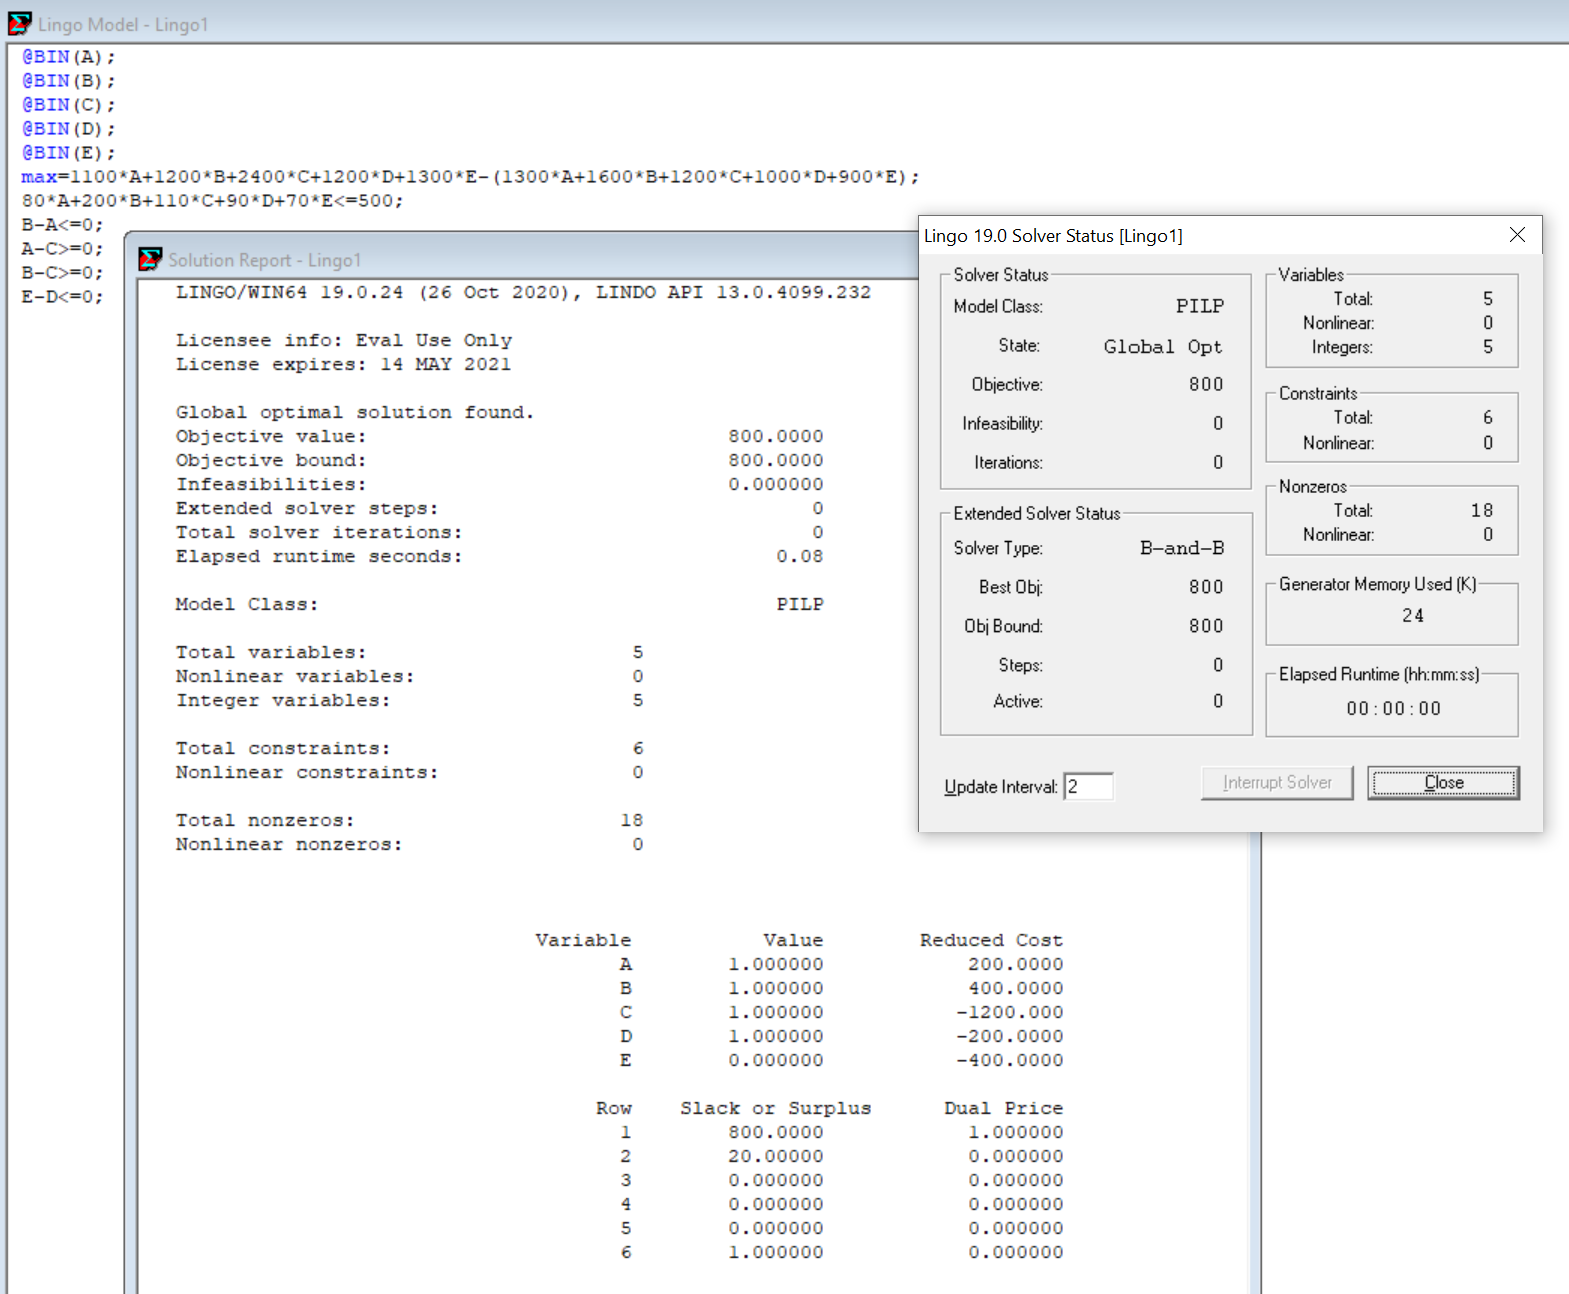
\includegraphics[width=1\linewidth]{src/blatt_6_aufgabe_3_solverloesung.png}
\end{centering}

\vspace{6mm}

Bei der Optimallösung werden die Gebiete A, B, C, D für den Erdgasnetzausbau erschlossen. Das Gebiet E wird nicht erschlossen. Es bleiben 20 Tage Bauzeit ungenutzt (Row 2) und es ergibt sich ein Gewinn von 800 TEuro.

\end{document}